\documentclass[11pt]{article}
\usepackage[utf8]{inputenc}\usepackage[T1]{fontenc}
\usepackage[a4paper,margin=2.3cm]{geometry}
\usepackage{amsmath,amssymb}\usepackage{booktabs}\usepackage{graphicx}\usepackage{hyperref}
\usepackage{xcolor}\usepackage{enumitem}
\graphicspath{{figures/}}
\title{A walk-holonomy controller, and why a Steiner design is its best structural basis}
\author{Cs.\ Hajdu \quad(with Claude Code)}
\date{2026-06-28 \quad\textit{Status: toy-scale, supervised --- promising, not yet closed-loop}}
\begin{document}\maketitle

\paragraph{One line.} A controller whose internal structure is a \emph{combinatorial design} can replace iterative
graph message-passing with a \textbf{single static gather along the design's walks} --- reaching the same
structural accuracy at $\sim$10$\times$ less compute --- and a \textbf{balanced Steiner design is measurably the
best such structure}.

\section{The idea}
Our signed-graph controller (HSiKAN) propagates signals layer by layer --- many small spline operations, slow
($\sim$2.8\,ms/forward, launch-bound). But over a \emph{fixed} topology the relevant structural features are the
graph's signed walks/cycles, which can be enumerated \textbf{once}. The forward then collapses to: gather node
features along the walks weighted by the \textbf{sign-product} (the $\mathbb{Z}_2$ \emph{holonomy} --- parallel
transport along the walk), scatter to each node, read out. No message-passing. We call this the
\textbf{StructuralActor}; algebraically it is one precomputed operator $B^{L}$ (the signed $L$-hop adjacency power)
applied to the input. The generated design hypergraphs are shown in Figure~\ref{fig:hg}.

\begin{figure}[h]\centering
  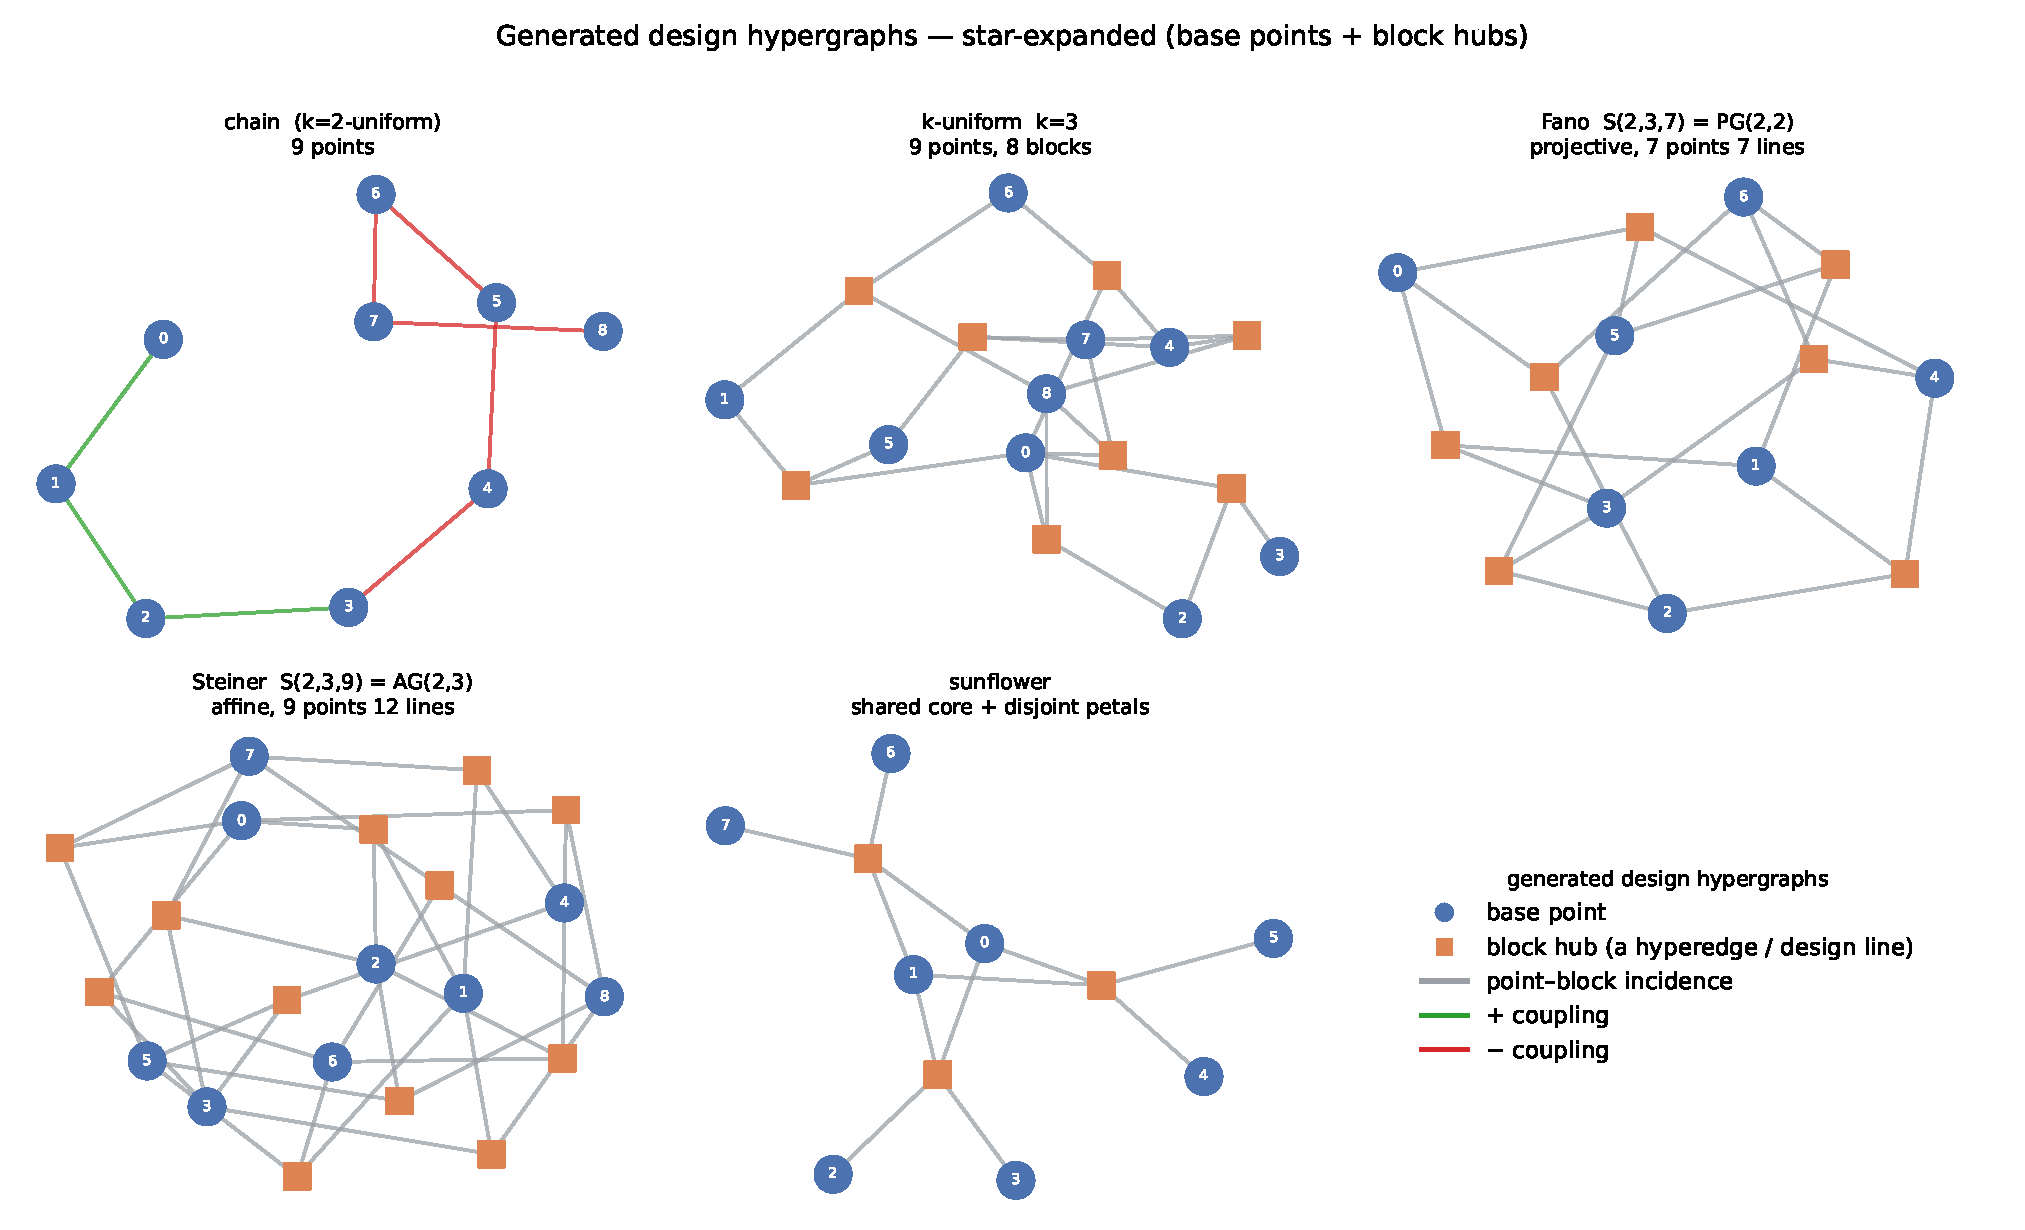
\includegraphics[width=\textwidth]{design_hypergraphs.pdf}
  \caption{The generator family as star-expanded hypergraphs: blue circles are base points, orange squares are
  block hubs (each hub = one hyperedge / design line), grey edges the point--block incidence. Chain is the
  $k{=}2$-uniform case; Steiner $S(2,3,9)$ is the affine plane AG(2,3) (every pair of points on exactly one line).}
  \label{fig:hg}
\end{figure}

\section{Measured ($N{=}9$, supervised, structural target; median over seeds)}
\begin{center}\begin{tabular}{lccc}
\toprule
generator & StructuralActor & HSiKAN & MLP \\
\midrule
chain ($k{=}2$-uniform) & 0.009 & 0.007 & 0.055 \\
$k$-uniform ($k{=}3$)   & 0.021 & 0.0006 & 0.037 \\
\textbf{Steiner $S(2,3,9)=$ AG(2,3)} & \textbf{0.0008} & 0.0004 & 0.031 \\
sunflower               & 0.017 & 0.0012 & 0.022 \\
\bottomrule
\end{tabular}\end{center}

\noindent Latency: StructuralActor $\sim$230--280\,$\mu$s vs HSiKAN $\sim$2600--3100\,$\mu$s ($\sim$10$\times$),
at 73 vs 2209 parameters. Three measured facts (see Figure~\ref{fig:acc}):
\begin{enumerate}[nosep]
  \item The actor matches HSiKAN's structural accuracy at $\sim$10$\times$ lower latency and $\sim$30$\times$
        fewer parameters. The key was the \emph{holonomy} (sign-\textbf{product} transport), not a signed sum ---
        a $\sim$95$\times$ accuracy jump from that one change.
  \item The \textbf{balanced Steiner design is the best structural basis} (0.0008), an order tighter than the
        $k$-uniform designs --- ``every pair coupled exactly once'' gives a non-redundant walk basis.
  \item It must enumerate \emph{enough} walks; at scale this becomes a scored top-$K$ (balanced designs need
        fewer walks for the same coverage --- another point for Steiner).
\end{enumerate}

\begin{figure}[h]\centering
  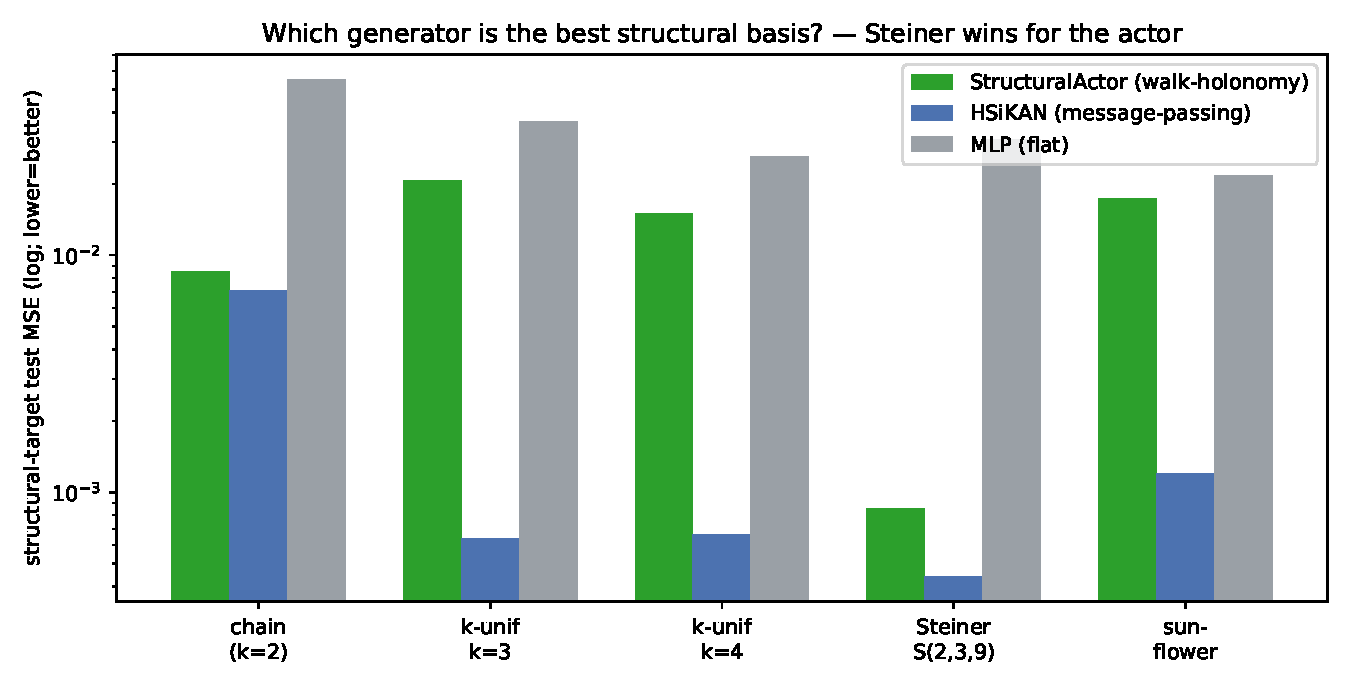
\includegraphics[width=0.82\textwidth]{generator_accuracy.pdf}
  \caption{Structural-target test MSE per generator (log scale). The StructuralActor (green) tracks HSiKAN (blue)
  and beats the MLP (grey) everywhere; the Steiner design gives the tightest actor fit.}
  \label{fig:acc}
\end{figure}

\section{Why this connects to deeper mathematics (conjecture, testable)}
The structure is a \textbf{principal bundle}: a flat, bounded \emph{finite affine geometry} (the base, AG(2,3))
carrying a \emph{connection} whose \textbf{holonomy} supplies the nonlinearity. In increasing order of how
testable the link is:
\begin{itemize}[nosep]
  \item \textbf{Discrete differential geometry} --- signed graph $=\mathbb{Z}_2$ connection; walk $=$ parallel
        transport; cycle holonomy $=$ curvature; balance $=$ flat connection. $B^{L}$ is the connection-Laplacian.
  \item \textbf{Clifford / geometric algebra} --- the transport generalises $\mathbb{Z}_2$ signs $\to$ SO(3)
        rotors ($\mathrm{Spin}(3)=\mathrm{Cl}^{+}(3,0)$) $\to$ multivectors; the rotor / geometric-attention line
        is the same ladder one rung up.
  \item \textbf{Frame theory (the falsifiable one)} --- Steiner systems construct \emph{equiangular tight frames}
        (Fickus--Mixon--Tremain, 2012). Candidate explanation for ``Steiner is best'': its blocks form a
        \textbf{tight frame} (optimal, minimal-coherence). \emph{Discriminating test:} does a design's frame
        coherence predict the actor's accuracy? If yes, ``balanced 2-design $=$ optimal control basis'' has a
        theorem behind it.
  \item \textbf{Geometric control / gauge theory of locomotion} --- control \emph{as} holonomy (geometric phase;
        Shapere--Wilczek). A gait that nets displacement from a cyclic shape change \emph{is} this; the
        walk-holonomy is its discrete analogue.
\end{itemize}
A nonlinear basis placed directly on the design's blocks (a block-wise \emph{Steiner-KAN}) curves the effective
geometry without a separate connection --- an alternative, more expressive construction worth comparing.

\section{Honest status}
Everything measured is \textbf{representation}, not closed-loop control: a supervised toy ($N{=}9$, one structural
target, two seeds). The architecture, the Steiner-is-best result, and the speed are real and reproducible; the
geometric-control reading is a \textbf{well-posed conjecture} until the holonomy readout is wired to actuators and
shown to \emph{control} a plant. Two cheap next experiments: (1) does frame coherence rank the generators (the
tight-frame theorem); (2) close a loop with a Steiner-structured actor on a balancing plant.
\end{document}
